% HMC Math dept HW template example
% v0.04 by Eric J. Malm, 10 Mar 2005
\documentclass[12pt,letterpaper,boxed,cm]{hmcpset}

% set 1-inch margins in the document
\usepackage[margin=1in]{geometry}
\usepackage{mathtools}
\usepackage{mathrsfs}
% include this if you want to import graphics files with /includegraphics
\usepackage{graphicx}
\usepackage{cases}
\usepackage{hyperref}
\usepackage{siunitx}
\usepackage{tikz}
\usepackage{cases}
\usepackage{mathalfa}
\usetikzlibrary{arrows}

% info for header block in upper right hand corner
\name{Name: ~~~~~~~~~~~~~~~~~~~~~~~~~~~~~~~}
\class{Physics 51}
\assignment{Homework \#23}
\duedate{December 5, 2016}

\newcommand{\ev}[2]{\Big|_{#1}^{#2}}
\newcommand{\evv}[2]{\Big|_{#1}^{#2}}
\newcommand{\set}[1]{\left\{#1\right\}}
\newcommand{\s}[1]{\sqrt{#1}}
\newcommand{\f}[2]{\frac{#1}{#2}}
\newcommand{\p}[2]{\frac{\partial #1}{\partial #2}}
\providecommand{\t}[1]{\text{#1}}
\providecommand{\span}[1]{\text{span}\left(#1\right)}
\providecommand{\set}[1]{\left\{#1\right\}}
\providecommand{\l}[0]{\left}
\providecommand{\r}[0]{\right}
\newcommand{\m}[1]{\begin{matrix}#1\end{matrix}}
\newcommand{\bm}[1]{\begin{bmatrix}#1\end{bmatrix}}
\renewcommand{\bf}[1]{\mathbf{#1}}
\newcommand{\pn}[1]{\left( #1 \right)}
\newcommand{\abs}[1]{\left| #1 \right|}
\newcommand{\bk}[1]{\left[ #1 \right]}
\newcommand{\cis}[1]{\pn{\cos\pn{#1} + i\sin\pn{#1}}}
\newcommand{\cisi}[1]{\pn{\cos\pn{#1} - i\sin\pn{#1}}}
\renewcommand{\Im}[1]{\text{Im}\pn{#1}}
\renewcommand{\Re}[1]{\text{Re}\pn{#1}}
\renewcommand{\k}[0]{\f{1}{4\pi\epsilon_0}}
\renewcommand{\part}[1]{\vspace{1em}\noindent(#1)}

\makeatletter
\renewcommand*\env@matrix[1][*\c@MaxMatrixCols c]{%
  \hskip -\arraycolsep
  \let\@ifnextchar\new@ifnextchar
  \array{#1}}
\makeatother
\begin{document}
\problemlist{Townsend 1.\{25*, 27, 29, 34\}}
	
\begin{problem}[Townsend 1.25*]
	Suppose that a thin film of acetone (index of refraction $n = 1.25$) of thickness $d$ is coating a thick plate of glass (index of refraction $= 1.50$). Take the magnitude of the amplitude for reflection of a photon from the top or the bottom surface of the acetone at normal incidence to be $r$ and assume that there is an additional phase change of $\pi$ in the reflection from the top and the bottom surface of the acetone, since at each of these surfaces light is passing from a medium with a lower index of refraction to one with a higher index of refraction. Calculate the probability that a photon of wavelength $\lambda$ reflected. Assume that amplitudes that involve multiple reflections at the bottom surface of the film can be neglected in your calculation. Express your answer in terms $\lambda$ and $r$ as well as the thickness $d$ and the index of refraction $n$ of the acetone. What is the minimum thickness of the coating necessary to produce zero reflection? \textit{Note}: For the air-acetone and acetone-glass surfaces $r \cong 0.1$.
\end{problem}
\begin{solution}
\end{solution}
\newpage

\begin{problem}[Townsend 1.27]
Figure 1.43 shows a Michelson interferometer with a movable mirror $M_1$, a fixed mirror $M_2$, and a beam splitter $M_s$ which is a half-silvered mirror that transmits one-half the light and reflects one-half the light incident upon it independent of the direction of the light. The source emits monochromatic light of wavelength $\lambda$. There are two paths that light can follow from the source to the detector. as indicated in the figure. Note that path 1 includes travel from the beam splitter $M_s$ to the movable mirror $M_1$ and back to the beam splitter, while path 2 includes travel from the beam splitter $M_s$ to the fixed mirror $M_2$ and back to the beam splitter. Assume the beam splitter introduces a phase change of $\pi$ for light that follows path 1 from the source to the detector relative to light that follows path 2 from the source to the detector. Also assume the mirrors $M_1$ and $M_2$ reflect 100\% of the light incident upon them and the photodetector PM (a photomultiplier) is 100\% efficient as well. 
\begin{enumerate}
	\item[(a)] Use the principles of quantum mechanics to determine the probability that a photon entering the interferometer is detected by the photodetector. Express your answer in terms of the lengths $l_1$, $l_2$ and $\lambda$. 
	\item[(b)] Find an expression for $l_1$ in terms of $l_2$ and $\lambda$ such that there is 100\% probability that the photon is detected by the photodetector. 
	\item[(c)] Suppose that the movable mirror is shifted upward by a distance $\lambda/6$ from the position(s) that you determined in part(b). Find the probability that the photon is detected at the photodetector in this case.
\end{enumerate}
\begin{center}
	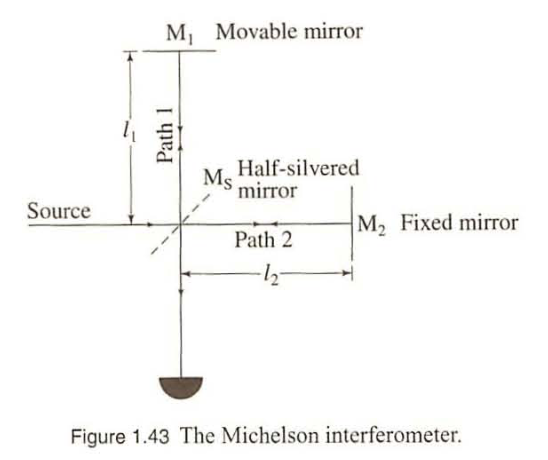
\includegraphics[scale=0.6]{pic1.png}
\end{center}
\end{problem}
\begin{solution}
\end{solution}
\newpage

\begin{problem}[Townsend 1.29]
Suppose that the two very narrow slits (widths $\ll \lambda$) in the double-slit experiment are not the same width and that the probability amplitude for a photon of wavelength $\lambda$ to strike a photomultiplier centered at a particular point P in the detection plane that makes an angle $\theta$ with the horizontal from one of the slits is larger by a factor of $\s{2}$ than for the other slit. Determine the visibility
	\[
		V = \f{P_\text{max} - P_\text{min}}{P_\text{max} + P_\text{min}}
	\]
	of the interference fringes, where $P_\text{max}$ is the maximum probability and $P_\text{min}$ is the minimum probability that a photon is detected.
\end{problem}

\begin{solution}
\end{solution}
\newpage

\begin{problem}[Townsend 1.34]
Starting from first principles, show that the probability that a photon of wavelength $\lambda$ hits a photomultiplier centered on a point P in the detection plane that makes an angle $\theta$ with the horizontal for a grating composed of three very narrow slits each separated by a distance $d$ is given by
\[
	\text{Prob} = r^2\pn{1 +4\cos\phi + 4\cos^2\phi}
\]
where $r^2$ is the probability that the photon would strike the photomultiplier with a single slit open and $\phi = kd\sin\theta = 2\pi d\sin\theta/\lambda$.
\end{problem}
\begin{solution}
\end{solution}

\end{document}